\chapter{5. Discussion}

This chapter discusses the implementation of the bikebump application and the
factors requiring consideration when creating a collective urban design tool
that effectively engages the community.

\section{A generalized tool for collective urban design}
We have been investigating a new tool for having a bottom up urban design method.
The bikebump application concentrated on having two basic elements of design,
each having two sections within them. These four elements will be the building blocks
of a mobile community engagement tool for collective urban designing.
The following will cover the design decisions that each component should consider.

\subsection{Analytic Phase}
The analytic phase is where the community learns the current situation in two dimensions. One is the individual level, where they experience the road themselves. Paying attention to the road condition changes the way they think while riding.
\footnote{18 out of 20 people said the application made the subject aware about the road condition.}
These individual experiences gather and compile into a collective view. Users can interpret the results relative to what they felt while riding. This aspect is different from when only the urban planning professionals draft the plan, often only looking at the visualization.

\textbf{1. data collection} \\
Bikebump used the DINGs as a method to collect data. As an urban design tool retrieving the geolocation data from devices will be mandatory. Deciding what other data to collect changes how much
we count on the humans as sensors. We could make the decision to record the sound of the whole commute and process it afterwards. This relies more on the sensors themselves and the assumption of what kind of sound people think is dangerous. Methods that fall in the same category vary in what kind and how much rich information we collect.

The application might record accelerometer data to detect places where people suddenly change speed, or take a video to later process to image recognition techniques. The other aspect is the human sensor, which for bikebump was the act of people ringing the bell for reports. The experiment explicitly did not specify the definition of ``good''/``bad'' except mentioning this was an attempt to improve bike lane security. \footnote{This is a design decision whether the experiment focuses on human perception, which is often ambiguous signals different from exact readings from mechanical sensors.}
Alternative to this approach a simple button to collect the perception.
\footnote{Within in the iteration of development button input was considered, but has been rejected for two reasons. One, it was dangerous to have people interact with their phones when they think it is already dangerous, thus having biased data. Very few people ride their bikes with bare hands in winter.}

The black box may remain a black box whether we combine the sensor data and try to correlate the two methods of data acquisition, but advances on extended intelligence\cite{pubpub:extended} may lead to accurate predictions of people's perceptions. The difficulty of this is the human sensors adjust to the environment and previous experiences. Cities with a lot of safe bike lanes may be very sensitive to small issues, relative to places that do not have much bike safety infrastructure. Not only that the app itself may change the behavior of reporting, after knowing the synthetic phase, people will digest the experience and adjust the definition of ``good''/``bad''.

\textbf{2. visualization} \\
The visualization was what the subjects observed after different kinds of data were processed. The main difference between other visualizations is the purpose. Attempts that end as a visualization is to give the observer an insight of a what the data shows. In addition to this, the visualization for a collective design tool should bridge the synthetic phase and what people have proposed. This means at least two different types of information will be superimposed: the result of the data collection phase and what was proposed to improve the place.

Bikebump visualized the consecutive GPS readings throughout the commute to show where people have actually passed. This will be a mechanism for balancing the improvement plans, since the number of DING reports may not always align to the trips taken.


\subsection{Synthetic Phase}
The RVSP cycle is a design process that is not constrained by the order of each R, V, S, and P phase. Alexander clearly mentioned the order of the analytic phase coming first.


One remark from the user test was the application is too organized toward being a linear process, which the user may not always follow. The application does not force the process to be completely linear, 
\footnote{There was a constrain of the order for proposing. An improvement plan was only able to be created if the ROAD had at least one DING report associated.}
\hlcyan{but the accessibility of these functions\footnote{report, view map, propose, vote} could have been weighted according to the usage frequency of an average user.} The application did not take this into account and it remains an open question, since the objective of each user may differ, and may change each time. Consequently, this may be one reason this kind of collective urban planning tool should remain separate from the analytic phase and the synthetic phase. Yet there is still the possibility that without the analytic phase, the synthesis phase would be biased towards subjective preferences.

Compared to various analytic phases that show visualizations and provide understanding, a structured synthetic phase has not been around. People may not be aware of the reason; thus, additional incentives may need to be considered, covered in p.\pageref{sec:incent}

\textbf{3. solution creation} \\ 
This section is the most mentally demanding section of the application. \hlcyan{It suggests the main findings was the reality that subjects doubted that their actions would have a real-world effect. They did not know how start interaction in the first place.} In addition, the interface tends to be the most complicated because the amount of information it handles is large. In bikebump, the users had to look for the road and its region, and match the specific SOLUTION type. This section could be more constrained, limiting the possible solutions, for example, to only one solution.\footnote{Ex. Just painting the road.}
\hlcyan{The key factor to show that their input will influence the process is outside of the design of the application, but rather building social norm that the application will make changes.}

\textbf{4. prioritization} \\
This phase can be interpreted as a collective sorting phase, where people use their own mind to order the improvement plans submitted by others. This phase is less demanding compared to the solution creation section, but the interface should be carefully structured, as this is where the judgment happens. Given the fact that this tool will always have geolocation, and sorting is the act of reordering the list, it is natural to have it plotted in a map and a list. In this case, the method for how the system sorts the list is an important factor to consider.

\subsection{How to tackle ``relative'' valuing}

One finding is the reports are ``relative'' to the previous experience. This is another characteristic of the `wicked problem', which `wicked problems' are essentially unique. \hlcyan{There may be overlapping contexts for each situation, yet does not guarantee that a single difference overrides the importance and influence the decision. The intersection where Beacon street changes to Bay State Rd, was showing the relativity of the timing of intervention and the location. The experiment was after the upgrade of beacon street, which is different thinking an intervention without that improvement, similarly it deforms the issue knowing that there is a safe road before that and the gap is the dominant aspect in consideration.}
\cite{rittel1973dilemmas}
It is unique since each user may have different perceptions on bike lane security, but more importantly, it is relative to the previous set environment.

Multiple people commented on the relativity of their perception. Data shows they felt insecure when bike lanes disappeared,
\footnote{The intersection of Beacon Street and Bay State Street, which the separated bike lane disappears. This separated bike lane was installed in response to a bike accident.}
\hlcyan{Despite this perception of unsafety, we do not know whether overall safety has actually decreased}

The users’ feedback also cast new questions on how to annotate the city. Bikebump used a 15m radius geofence as a method, but users implied that ``good'' situations were likely to be a continuous experience rather than a moment reaction. Measuring methods looking at a constant input may also validate this perception

\section{Incentives for bottom Up design, do we care?}
\label{sec:incent}

It is likely that bikers are aware that the city is still dangerous and needs improvements. Yet none of the subjects know the interventions the city is contemplating.

One reason may be that the mental threshold of changing their city is so costly that they do not even bother learning how to inspire the city to make changes or \hlcyan{may be that these procedures are bureaucratic and opaque and hard for people to acknowledge}.

This might be supported by the fact that younger people tend to moving more frequently, which whether you devote for any participatory design, you will be living somewhere else by the time you are able to appreciate the physical change.
\footnote{It is apparent that younger people move more than the elder generations. 
\url{https://fivethirtyeight.com/datalab/how-many-times-the-average-person-moves/}
, yet there are reports that the rate of younger people moving is decreasing over time.\\
\url{http://www.nytimes.com/2012/03/11/opinion/sunday/the-go-nowhere-generation.html}
}

Shorter span reward is preferable, and it may be preferable for different reasons. We can see this by the
loop of dopamine coming from the instant gratification from peer approval on social media networks.

While this thesis stands on the fact that the application or website is already recognized by the user,
it is important to consider how to design the initial contact.

\subsection{Initial Contact with citizens}

\textbf{Where} \\ 
In the after-bike discussion, more than half of the people said that they preferred not to have the city supervising or the planning side set a concentration area for getting input. People demanded an open platform that they report, propose, and vote whenever and wherever they wanted. On the other hand, people also recognized that if that were the case, \hlcyan{the likelihood of overlapping events being registered by the app would be totally by chance}. This creates possibilities for how we recruit participants. It is easier to start from a trial that has a target path, meeting the need from the city, and to gradually expand to a greater audience. This is possible, because of the mobile characteristics of the application, and is unique compared to the traditional methods of community engagement.


\textbf{When} \\
Methods that require people to meet physically has a limit to the physical space but time is also a constrain. It is hard to coordinate these two and have the majority of the people building consensus. The application can be installed and used anytime, yet the capacity of human cognition in a given time is also limited. A survey shows that most of the Android applications lose 77\% of the daily active users after three days.
\footnote{\url{http://andrewchen.co/new-data-shows-why-losing-80-of-your-mobile-users-is-normal-and-that-the-best-apps-do-much-better/}}
It is also true that even in the cases of the most dreadful natural disasters, we easily lose interest in after a short period of time. \hlcyan{Figure \ref{fig:tohoku_trend} shows this trend, yet we can see that people recall the disaster every year which is an attempt to delay being forgotten.}

\begin{figure}[!htb]
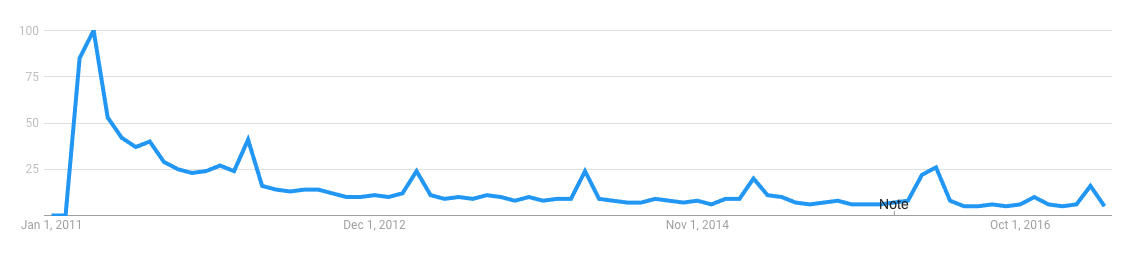
\includegraphics[\textwidth]{chapters/5/fig/tohoku_trend.png}
\caption[Trend for North East Japan Tohoku Earthquake]{\textbf{Google Trend} number of searches for the term `North East Japan Tohoku Earthquake'. We see a sharp degrade after the disaster, but periodic pulses occurs every year maintaining attention.}
\label{fig:tohoku_trend}
\end{figure}

The proposed process to incorporate Bikebump in the current TIP method still has an annual cycle to update the list of demanding improvement proposals. 
Rather than releasing the application and waiting for the community to spontaneously participate, a periodic campaign may be effective.
If we think of the attention from the public as something we need to raise, a report from the Nonprofit Research Collaborative
\footnote{\url{https://npresearch.org/pdf/2014-reports/NRC_AnnualFund_SpecialReport_July_2014.pdf}}
also points out that nonprofit organizations tend to meet their fundraising goals from annual funds.

\subsection{Communal value to Civic value}
Shirky points out that the internet has lowered the threshold barrier to coordinating with each other,
and within this collective action,
there are two kinds of value mechanisms; communal and civic values. \cite{shirky2010cognitive}

Communal value is created and acknowledged by the same group. \hlcyan{On the other hand, civic values may be created by a small group but acknowledge by the whole society.} Although bikebump targets modification in
infrastructure, it is fundamentally by bikers that benefit the same group, which makes bikebump's engine the communal value behavior. \hlcyan{It is different from examples like Wikipedia, which the authors and editors of posts is substantially small compared to the group that benefits from their effort.}

One comment from the user test was the personalization of the application.
The application did not show identity.
\footnote{except distinguishing individual proposals.
One concern that users will be able to identify other users homes.} 
Waze uses icons to show other users in the map, aiming for the sense
of community within the people who drive in the same area.
Personalizing the application interface may make the user feel
more attached to the application, and emphasize the sense of a collective effort.

Allowing others using different modes of transportation is the next step for inclusion. For the analytical phase, \hlcyan{drivers and pedestrians could have an application that lets them give feedback on when they felt endangered, or had a close call with a bicyclists. By enabling small but all kinds of individuals participate, the civic value will increase.}

\section{Micro owning and share economy}

Focusing on bike lanes, bikebump was one utilization of
the collective urban planning tool. \hlcyan{Despite the existence and successful testing of this platform, it is impossible to extrapolate and conclude that this method will work for other aspects of urban infrastructure.} 
\footnote{For specific applications, refer to the future work (p.\pageref{sec:future}) section in chapter 6.} \hlcyan{To have this method applied to other urban planning issues, these applications may need to change the social norm of how we own the city.}

We see the traces of the commutes from the map visualization generated from the users.
Although this was initially added to see how the commutes were \hlcyan{concentrated},
we can have another perspective that this is the traces of micro possession.

From the popularity and rise of mobile phones, there is a particular group of services that have been emerging; share economy related services. These new mobile-dependent services
\footnote{Car ride share and bike share services are obvious, but also Airbnb does not let you book without
a smart phone, Android tablet, or an iPad.
\url{https://community.withairbnb.com/t5/Hosting/How-to-accept-reservations-via-cell-phone-but-wittd-p/11129}}
are anticipated to be disruptive innovations that especially make the cities’ resources efficient.

Yet urban areas have been a sharing space for a long time. Restaurants are shared places to eat food.
Parks are shared areas which cities maintain using tax income. Infrastructure like roads should be included as well.
The only difference is that the parks and infrastructure are publicly operated by the government, it is owned by no one but everyone.
In contrast, new shared economy services ``share'', meaning users temporarily claim partial ownership. Without the support of these mobile applications, it is too risky thus the administrative cost is too expensive to maintain a ride sharing services without peer monitoring. The services leverages the computation the crowd holds to distribute opportunities for each member. As a result the services enables people to coordinate, negotiate, and ensure fair and transparent business.

We can say that a person who rents a bike from a bike sharing service owns the bike within the ride, but in addition, he also owns a fraction of road infrastructure within that very short time, which he then has the right to claim that his route should be safe. This is certain that when accumulated, commute routes become more ``yours'' than a place you never visited.
\footnote{This may be also taken as micro adverse possession, while currently it is not allowed to claim possession on public areas. Rose claims that the origin of property is possession.\cite{rose1985possession} The one who communicates the claim should in fact be rewarded with the property, because the act of clarifying property is already useful labor, that prevents costly conflicts thus facilitating trade.} \hlcyan{This leads to urban design not constrained with district levels but multi layers of partial ownership overlapped. The basic right for using the road may still be guaranteed, but the right to change the infrastructure to better suit the need will depend on who uses the road. It will be only within a prediction what will happen if this method was implemented, but we can guess the governmental scale will shrink in dense cities, since the ownership will fall in to regions that people can walk. If we see from Lessig's perspective, we can see this as a shift to ``market'' from ``law'', where the currency used for this market is the total time it was used.\footnote{Although it remains hypothetical, using time as the currency is fundamentally equal to everyone.} We see a city that is formed organically without a central government system much like the rich landscapes that Rudofsky's exhibition ``Architecture without Architects''} \cite{rudofsky1964architecture} presented. \hlcyan{To practically test this concept, one way maybe using a similar mechanism to Estonia's E-residency program. This program lets people create, own and maintain businesses without physically being at Estonia. In this micro owning case, we need a virtual government to grant rights to people who claim a portion of the city. Once being a virtual resident, the possession recording app will collect locations that the user passed or stayed, calculating where and how much the user owns in a microscopic way.}


